\setcounter{chapter}{4}
\chapter{数据通信技术基础}

数据通信是随着计算机技术与通信技术的迅速发展,以及两者间的相互渗透与结合而兴起的一种新的通信方式。在工业控制领域,随着工业生产规模的扩大和自动化水平的提高,越来越多的数据共享和消息交换需要通过数据通信解决。计算机控制系统中的数据通信指计算机与计算机之前间、计算机与仪器设备之间的数据交换。


\section{通信系统的性能指标}

通信系统的任务是传递信息,因而信息传输的有效性和可靠性是通信系统最主要的质量指标。


通信系统的模型为:


信息源 $\rightarrow d(t)$ 发送器 $\rightarrow s(t)$ 传输通道 $\rightarrow r(t)$  接收器 $\rightarrow d'(t)$  汇

\begin{remark}
由此模型可考虑以下问题:

\begin{enumerate}
  \item 接收到的数据d'(t)是否d(t)?
  \item 发送器及接收器的作用?具体是什么?
  \item 传输通道的具体形式?
  \item 如何衡量通信系统的性能?
\end{enumerate}

\end{remark}

\subsection{有效性指标}

\subsubsection{数据传输速率}

 包含以下两种:
  \begin{enumerate}
    \item 比特率

比特是数据信号的最小单位。
    通信系统每秒传输数据的二进制位数定义为比特率,记作bps。
    \item 波特率

波特是指信号大小方向变化的一个波形;把每秒传输信号的个数定义为波特率。
    单位: 波特(baud)。
  \end{enumerate}

\begin{remark}

波特率表示单位时间内信号波形的变换次数,即通过信道传输的码元个数。
若信号码元宽度为T秒,则码元速率B=1/T,单位叫波特。这是为了纪念电报码的发明者法国人波特(Baudot)。

1924年奈奎斯特推导出有限带宽无噪声信道的极限波特率,称为奈氏定理。若信道带宽为W,则奈氏定理的最大码元速率为:$B=2W (Baud)$

奈氏定理指定的信道容量也叫奈氏极限,它由信道的物理特性决定。超过奈氏极限传送脉冲信号是不可能的。因此要进一步提高波特率,就必须改善信道的带宽。

比特率指单位时间内信道上传送的信息量(比特数)。数字信道的通频带(即带宽)决定了信道中能不失真的传输脉冲序列的最高速率,即信道容量。在一定波特率下提高比特率的途径是让一个码元携带更多的信息量(比特数)。若把两比特编码为一码元,则数据速率可成倍提高,我们有公式:

\begin{equation}
R=Blog_2N=2Wlog_2N
\end{equation}

式中R表示比特率,B、N、W的含义如上所述,单位为每秒比特(bits per second),记为bps或b/s。

\end{remark}





  \begin{remark}

例如,有一个带宽为3kHz的理想低通信道,其码元传输速率为6000baud。而最高数据速率可随编码方式的不同而有不同的取值。若1 个码元能携带2bit的信息量,则最高的数据速率为12000bps。这些都是不考虑噪声的理想情况下的极限值。至于有噪声影响的实际信道,则远远达不到这个极限值。

  \end{remark}


  \subsubsection{协议效率}

协议效率是指所传输的数据包中的有效数据位与整个数据包长度的比值。通常用百分比表示。

  协议效率越高,其通信的有效性越好。
   通信参考模型的每个分层,都会有相应的层管理和协议控制的加码。从提高协议效率的角度来看,减少层次可以提高编码效率。


\subsection{可靠性指标}

  \textbf{误码率}是衡量数字通信系统可靠性的指标,是二进制码元在数据传输系统中被传错的概率,数值上近似:

  \begin{equation}
    P_e\approx N_e/N
  \end{equation}

N:传输的二进制码元总数;
Ne:为传输错的码元数

   \begin{remark}
     理解误码率应注意以下问题:
     \begin{enumerate}
       \item 误码率是衡量数据传输系统正常工作状态下传输可靠性的参数;
       \item 对于一个实际的数据传输系统,不能笼统的说误码率越低越好,要根据实际情况提出误码率要求;
       \item 实际数据传输中,往往需要进行大量的、重复的测试,才能求出平均误码率。
     \end{enumerate}


         据测试,电话线传输速率为$300-2400bps$时,平均误码率为$10^{-4} - 10^{-6}$,而计算机通信的平均误码率要求低于$10^{-8}$,因此,不采用差错控制,就不能满足计算机通信的要求。

   \end{remark}


\section{通信线路工作方式}


如图\ref{fig_5_01}所示,
  单工通信是指所传送的信息始终朝着一个方向,而不进行相反方向的传送。
  半双工(Half Duplex)通信是指信息可双向传输,但同一时刻只限于一个方向的传输。
  全双工(Full Duplex)通信是指能够同时进行双向数据通信。




\begin{center}
\begin{figure}
  \centering
  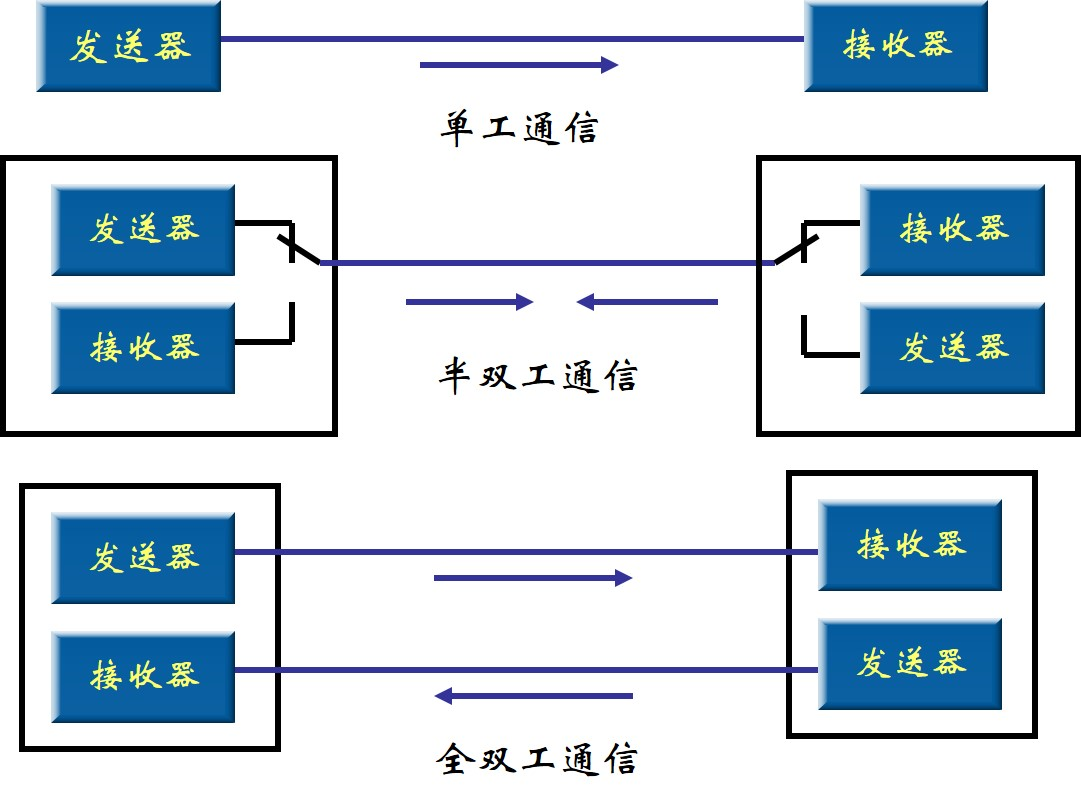
\includegraphics[width=0.6\textwidth]{fig_5_01}\\
  \caption{工作方式}\label{fig_5_01}
\end{figure}
\end{center}

\begin{remark}
举例:

  \begin{description}
       \item[单工] 广播电台,电台,单行路
       \item[半双工] 对讲机,USB 2.0,RS-485,分时段单行路
       \item[全双工] 电话,RS-232,USB 3.0,网络端到端通信(微信,QQ),一般道路
     \end{description}


\end{remark}

\section{传输介质与介质带宽}

\subsection{传输介质}

\textbf{传输介质}指数据通信中用来传递信号的媒体。例如,双绞线,屏蔽电缆,光纤。



\begin{center}
\begin{figure}
  \centering
  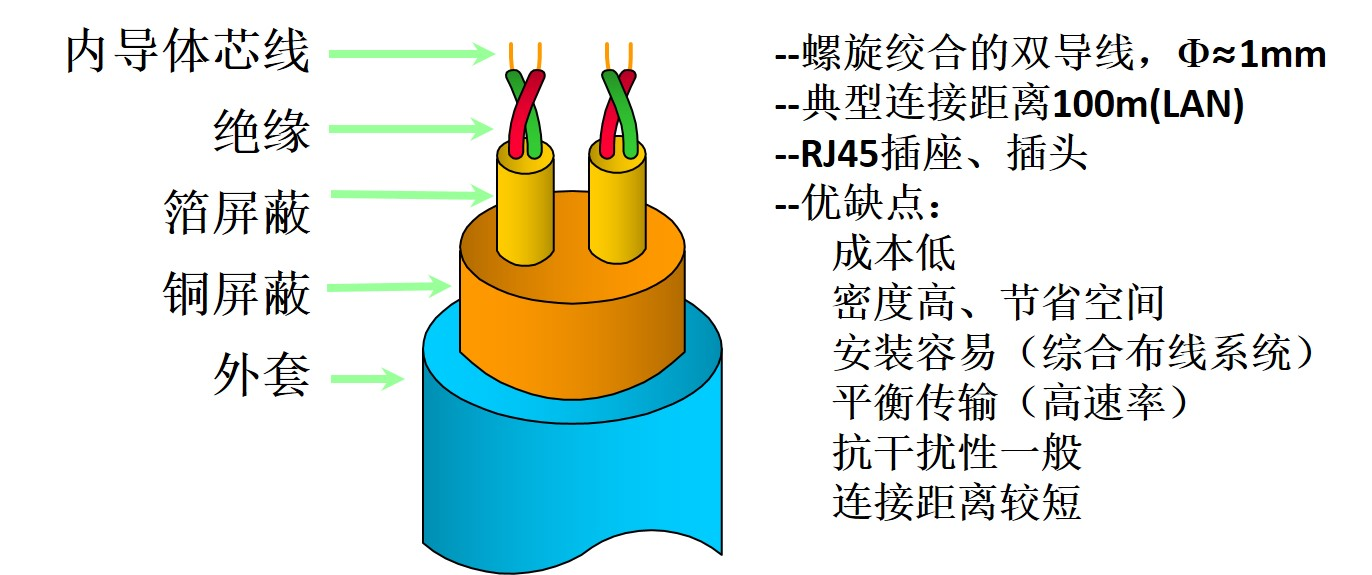
\includegraphics[width=0.55\textwidth]{fig_5_02}
  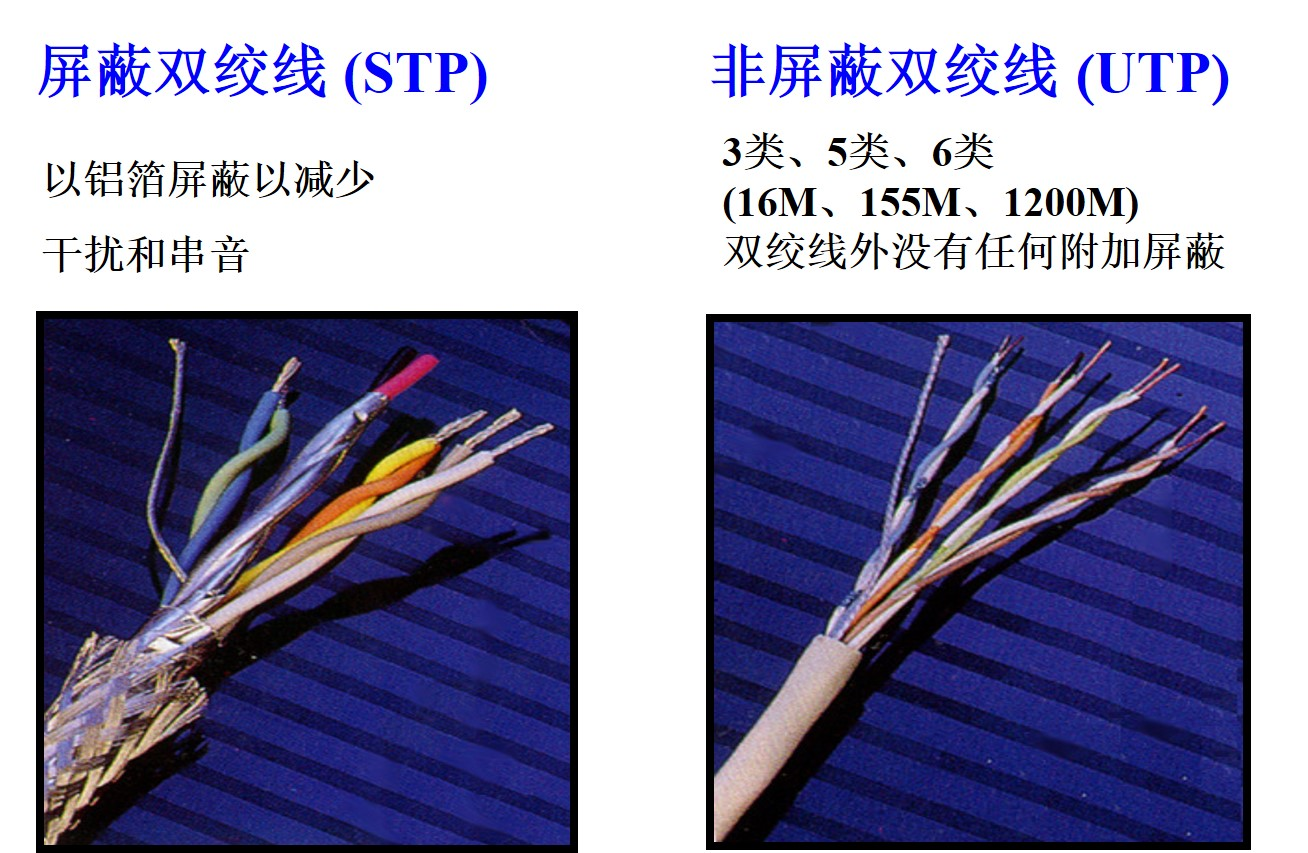
\includegraphics[width=0.40\textwidth]{fig_5_03}\\
  \caption{双绞线-(STP/UTP)}\label{fig_5_03}
\end{figure}
\end{center}



\begin{center}
\begin{figure}
  \centering
  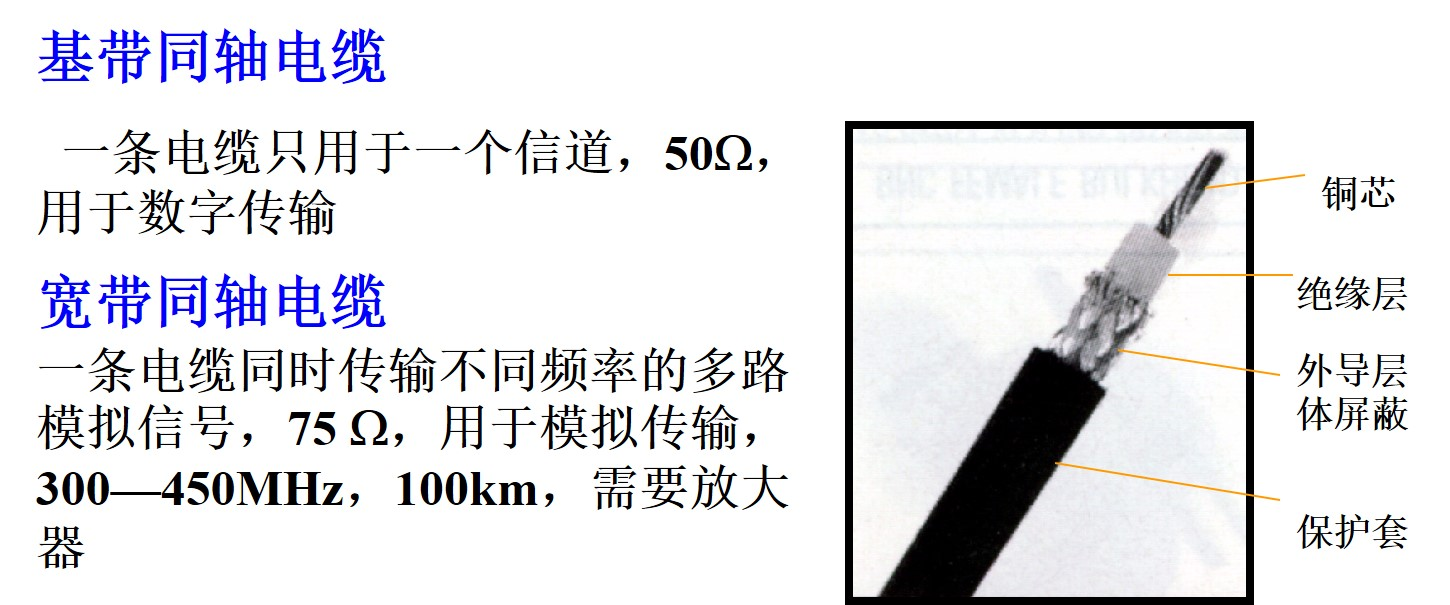
\includegraphics[width=0.6\textwidth]{fig_5_04}\\
  \caption{同轴电缆}\label{fig_5_04}
\end{figure}
\end{center}



\begin{center}
\begin{figure}
  \centering
  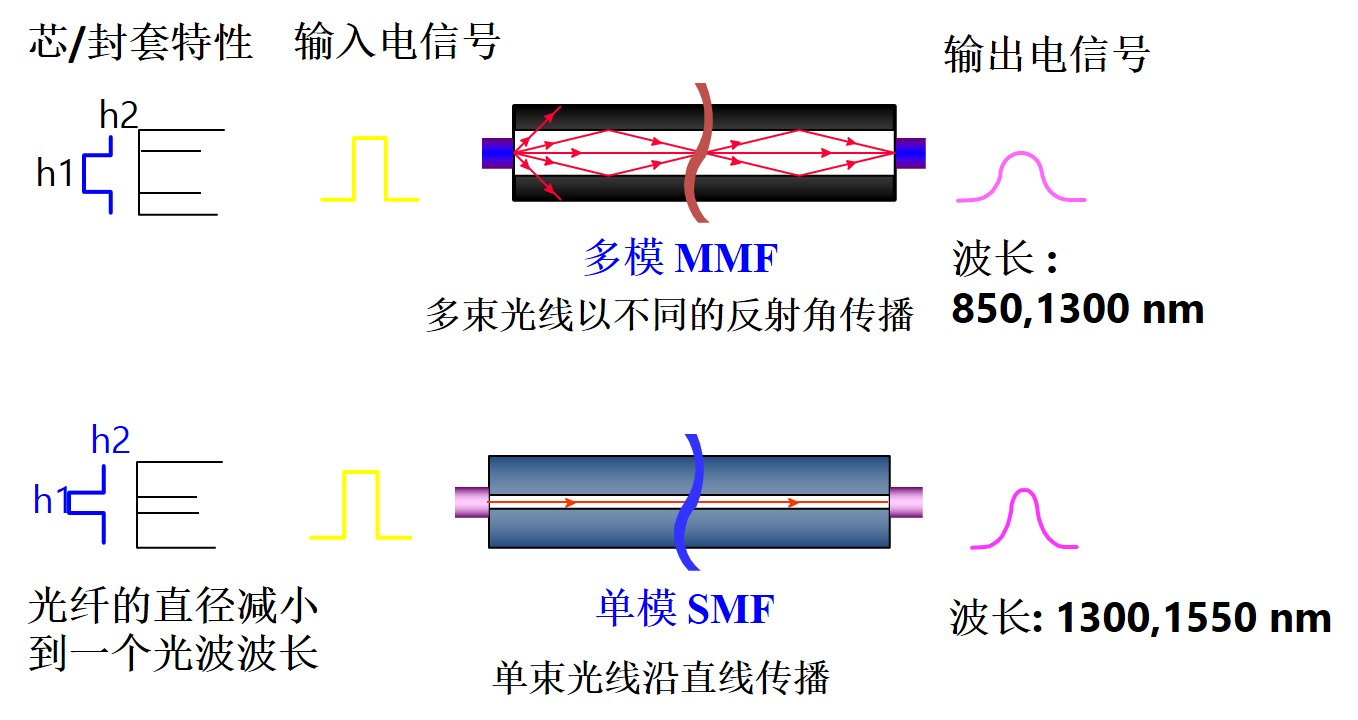
\includegraphics[width=0.55\textwidth]{fig_5_05}
  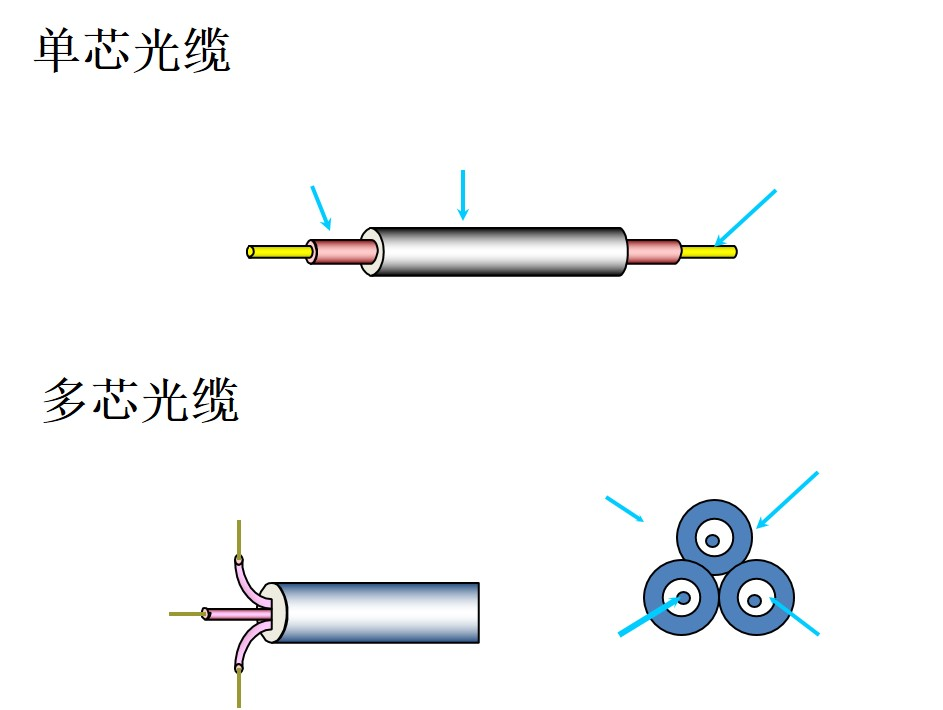
\includegraphics[width=0.40\textwidth]{fig_5_05a}
  \caption{光纤传送模式:MMF与SMF,单芯与多芯}\label{fig_5_05}
\end{figure}
\end{center}


\begin{remark}
光纤特点:直径小、频带宽、容量大、远距离高速传输、不受外界电磁干扰;成本相对昂贵、连接复杂
\end{remark}


\subsection{介质带宽}

不同的传输介质具有不同的带宽。


\begin{center}
\begin{figure}
  \centering
  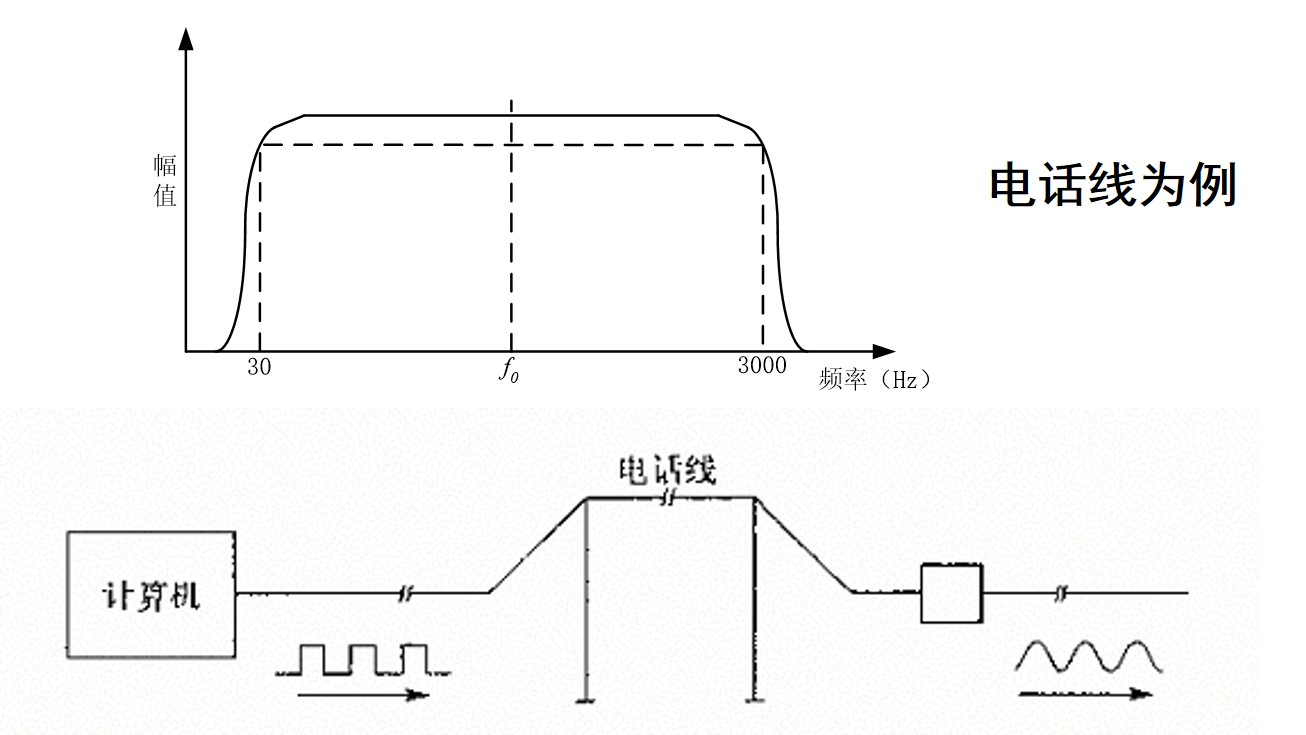
\includegraphics[width=0.55\textwidth]{fig_5_06}\\
  \caption{电话线的带宽}\label{fig_5_06}
\end{figure}
\end{center}

\begin{remark}
以电话线为例,如图\ref{fig_5_06}所示。
\begin{description}
  \item[信号带宽] 信号频谱的宽度,即信号的最高频率分量与最低频率分量之差。
  \item[介质带宽] 限定了允许通过该传输介质的信号的上、下限频率,也即一个频率能带。
\end{description}

情形1:如果信号与介质带宽相同且频率范围一致,信号能不损失频率成分地通过信道。
情形2:如果带宽相同,但频率范围不一致,则该信号的某些频率分量肯定不能完全通过该介质。

\end{remark}

\section{基带与载波传输}

\subsection{基带传输}

\begin{description}
  \item[基带传输] 在基本不改变数据信号频率的情况下,在数字通信中直接传送数据基带信号,即按数据波的原样进行传输,不采用任何调制措施。
目前,大部分计算机局域网都是采用基带传输。特点:
\begin{itemize}
  \item 信号按数据位流的基本形式传输,整个系统不用调制解调器。
  \item 基带信号包含很宽频率范围,不适合远距离传输。
\end{itemize}

  \item[数字数据的数字编码] 用高低电平的矩形脉冲信号来表示数据的0、1状态。

  数字编码的种类有:单极性码、双极性码、归零码、非归零码、差分码、Manchester编码等。工业通信中常用的是非归零码和Manchester编码,如图\ref{fig_5_07}所示。

\end{description}

\begin{description}
  \item[非归零码] 通过高低电平表示逻辑1和0,在整个码元期间都维持有效电平的编码。

\begin{itemize}
  \item
\textbf{优点}:能够比较有效地利用信道的带宽,这是最常用的编码之一。
  \item
\textbf{缺点}:存在直流分量,不具备自同步机制,必须使用外同步。
\end{itemize}

  \item[曼彻斯特编码] 在每个码元的中间都要发生跳变。接收端可将此变化提取出来作为同步信号,使接收端的时钟与发送设备的时钟保持一致。是工业数据通信中最常用的一种基带信号编码

\begin{itemize}
  \item \textbf{优点}:不需要外同步信号,不存在直流分量。
  \item \textbf{缺点}:需要双倍的传输带宽(即信号速率是数据速率的2倍)。
\end{itemize}

\begin{center}
\begin{figure}
  \centering
  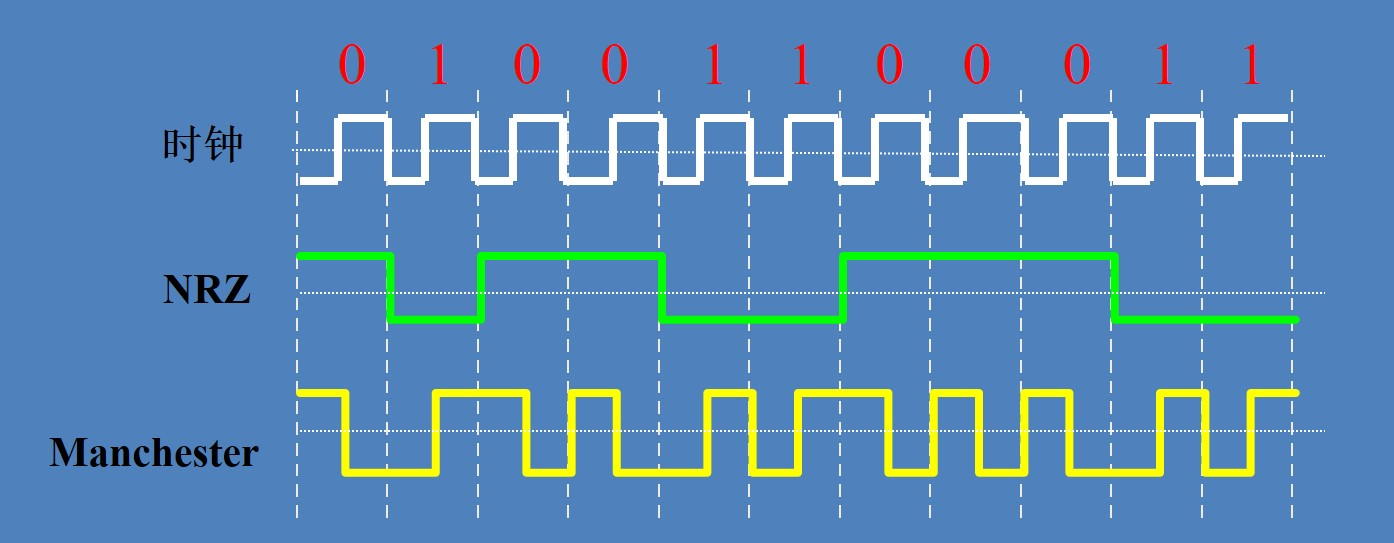
\includegraphics[width=0.55\textwidth]{fig_5_07}\\
  \caption{非归零码/曼彻斯特编码}\label{fig_5_07}
\end{figure}
\end{center}


\end{description}


\subsection{载波传输}

\begin{description}
  \item[载波传输] 是先用数字信号对载波进行调制,然后进行传输的传输模式。

  \item[基本原理] 用数字信号对载波$S(t)=Acos(\omega t+\phi)$ 的三个参量(幅度、频率、相位)进行调制,如图\ref{fig_5_08}所示。

  \item[常用技术] 包括:

  \begin{enumerate}
    \item 调幅: 幅移键控ASK(Amplitude Shift Keying)
    \item 调频: 频移键控FSK(Frequency Shift Keying)
    \item 调相: 相移键控PSK(Phase Shift Keying)
  \end{enumerate}

\begin{center}
\begin{figure}
  \centering
  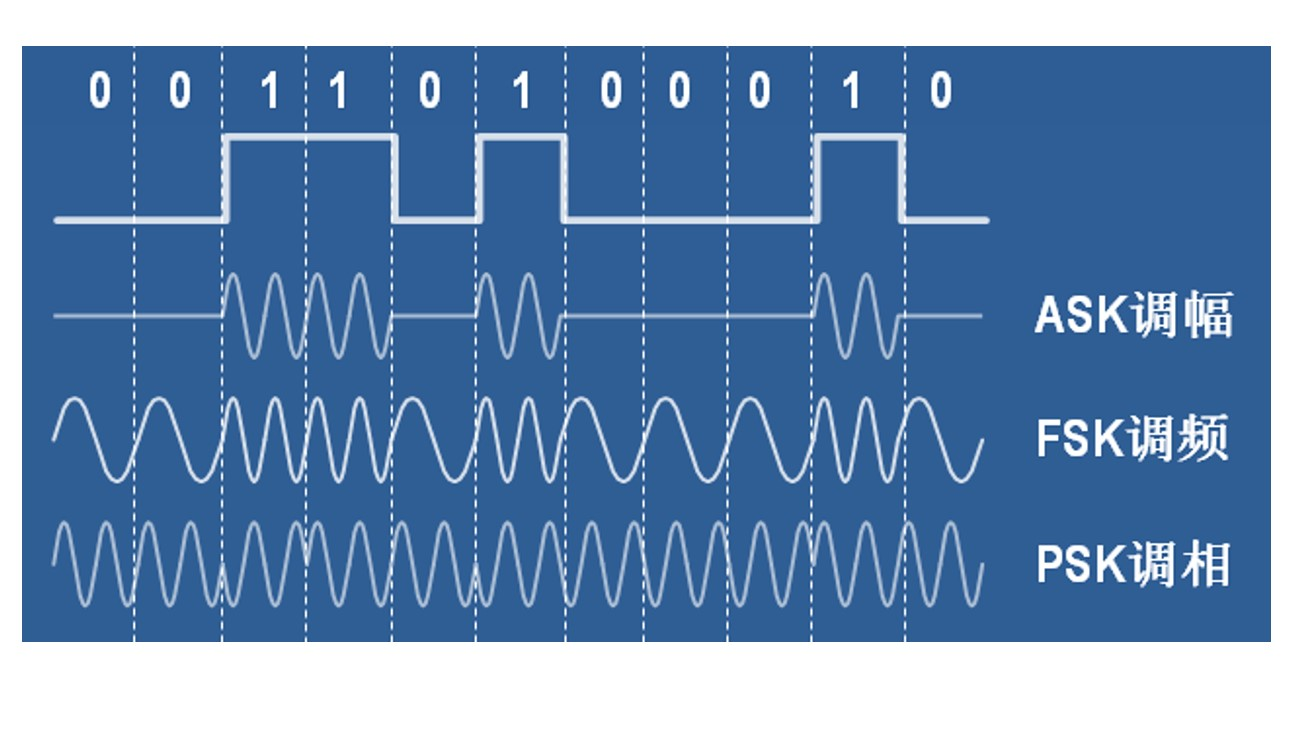
\includegraphics[width=0.55\textwidth]{fig_5_08}\\
  \caption{ASK/FSK/PSK}\label{fig_5_08}
\end{figure}
\end{center}

\end{description}



\section{通信数据的差错校验}
数据通信中,由于干扰等各种原因,数据差错不可避免,需要可靠判断出传输是否有误,即\textbf{差错校验}。

差错校验的\textbf{基本原理}是:发送方在发送数据基础上,生成某些\textbf{校验编码},附加在数据后面一起发送。接收方收到数据和校验码后,用校验码进行检验,确定本次传输是否出现错误。


\begin{description}
  \item[奇偶校验] 用这种校验方法,在发送时,在每一个字符的最高位之后都附加一个奇偶校验位。这个校验位可为“1”或为“0”,以便保证整个字符(包括校验位)为“1” 的位数为偶数(偶校验)或为奇数(奇校验)。接收时,按照发送方所确定的同样的奇偶性,对接收到的每一个字符进行校验,若二者不一致,便说明出现了差错。

      \begin{remark}
        ASCII码包含128个常用字符。因此,可用7b来表示其中的一个字符。在用ASCII码传递信息时,对其进行校验,如图\ref{fig_5_12}所示。

      \end{remark}
\begin{figure}
  \centering
  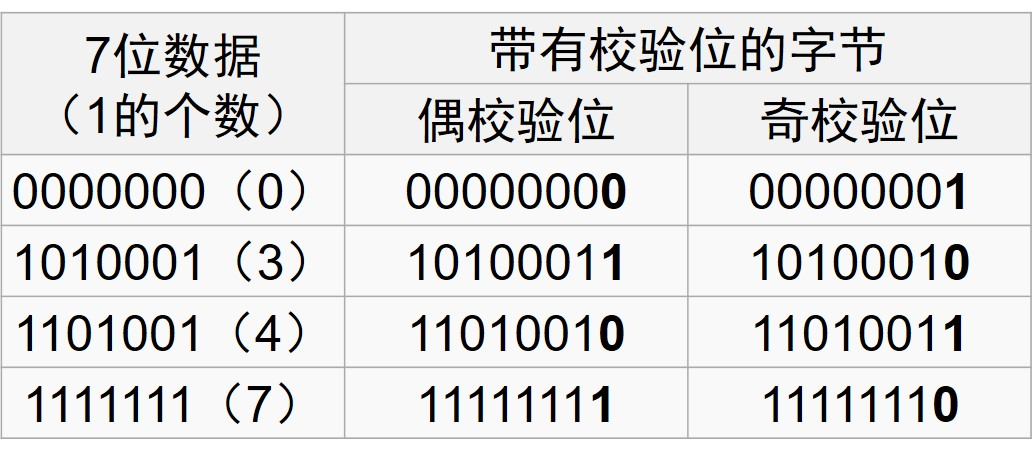
\includegraphics[width=0.4\textwidth]{fig_5_12}\\
  \caption{奇偶校验举例}\label{fig_5_12}
\end{figure}

\begin{remark}
  奇偶校验如何实现?异或运算(相异为1),即:

  $b_{check} = b1\bigoplus b2 \bigoplus b3 \bigoplus b4 \bigoplus b5 \bigoplus b6 \bigoplus b7 \bigoplus b8$

  对于01010101、11111111、00000000、00000001、00000011、11111110奇偶校验码分别为?
\end{remark}

  \item[校验和] 该种校验方法是针对数据块,而不是单个字符。在数据发送时,发送方对块中数据简单求和,产生一字节校验字符(校验和)附加到数据块结尾。校验和不能检测出排序错误。
\begin{figure}
  \centering
  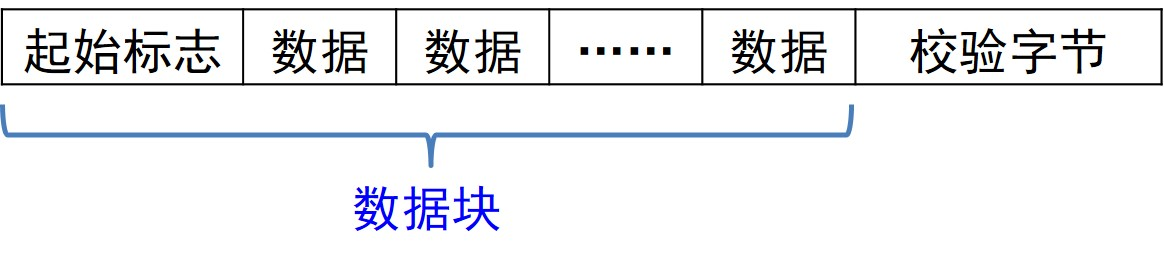
\includegraphics[width=0.55\textwidth]{fig_5_09}\\
  \caption{校验和}\label{fig_5_09}
\end{figure}
  \item[循环冗余码校验] CRC (cyclic redundancy code) 检错码方法是将要发送的数据序列当作一个信息多项式$f(x)$的系数,在发送方用收发双方预先约定的生成多项式G(x)去除,求得一个余数多项式R(x)。将余数多项式加到数据多项式之后发送给接收端。接收端用同样的生成多项式去除接收数据多项式$f'(x)$,得到计算余数多项式,然后进行比较。
  生成多项式由协议规定,目前已有多种生成多项式列入国际标准,如图\ref{fig_5_11}所示。

\begin{figure}
  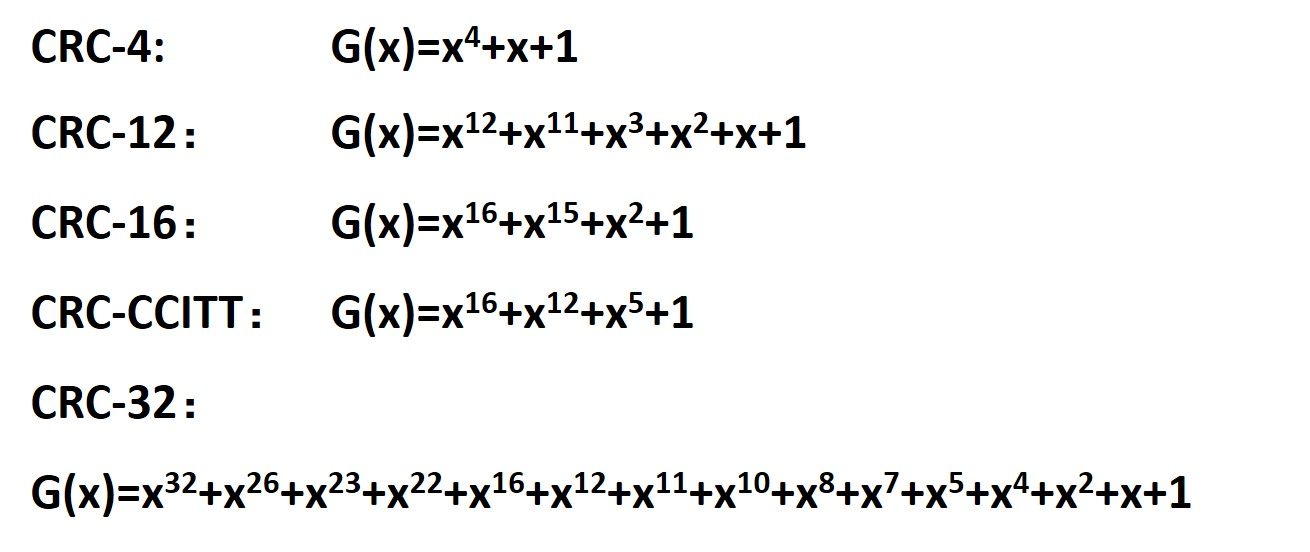
\includegraphics[width=0.48\textwidth]{fig_5_10}
  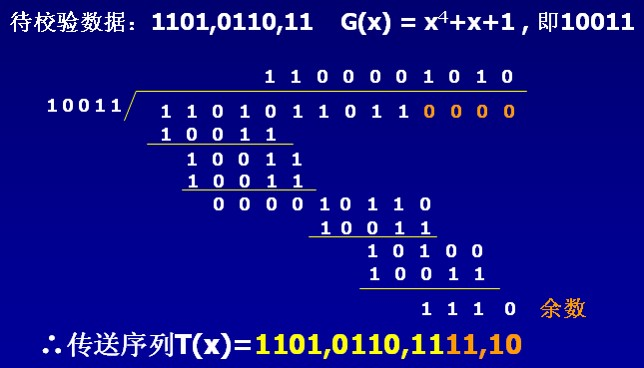
\includegraphics[width=0.48\textwidth]{fig_5_11}\\
  \caption{循环冗余码的种类和计算}\label{fig_5_11}
\end{figure}

\begin{remark}

\begin{itemize}
  \item 数据与多项式的对应关系;
  \item 余数的长度应为多少;
  \item 如何进行模2除法;
\end{itemize}
\end{remark}

\begin{remark}
模2除法:除法过程中用到的减法是模2减法, 不考虑加法进位和减法借位。只要部分余数首位为1,便可上商1,否则上商0。

\begin{verbatim}
0-0=0   0-1=1   1-0=1   1-1=0
\end{verbatim}

\end{remark}

\begin{remark}

例:如图\ref{fig_5_13}所示


\begin{enumerate}
  \item 发送数据比特序列为110011(6比特)。
  \item 生成多项式比特序列为11001(5比特,k=4)。
  \item 将发送数据比特序列乘以$2^4$,那么产生的乘积应为1100110000。
  \item 将乘积用生成多项式比特序列去除,按模二除法应为
  \item 将余数比特序列加到乘积中得1100111001

\item 如果在数据传输过程中没有发生传输错误,那么接收端接收到的带有CRC校验码的接收数据比特序列一定能被相同的生成多项式整除,即
\end{enumerate}


\end{remark}

\begin{center}
\begin{figure}
\centering
  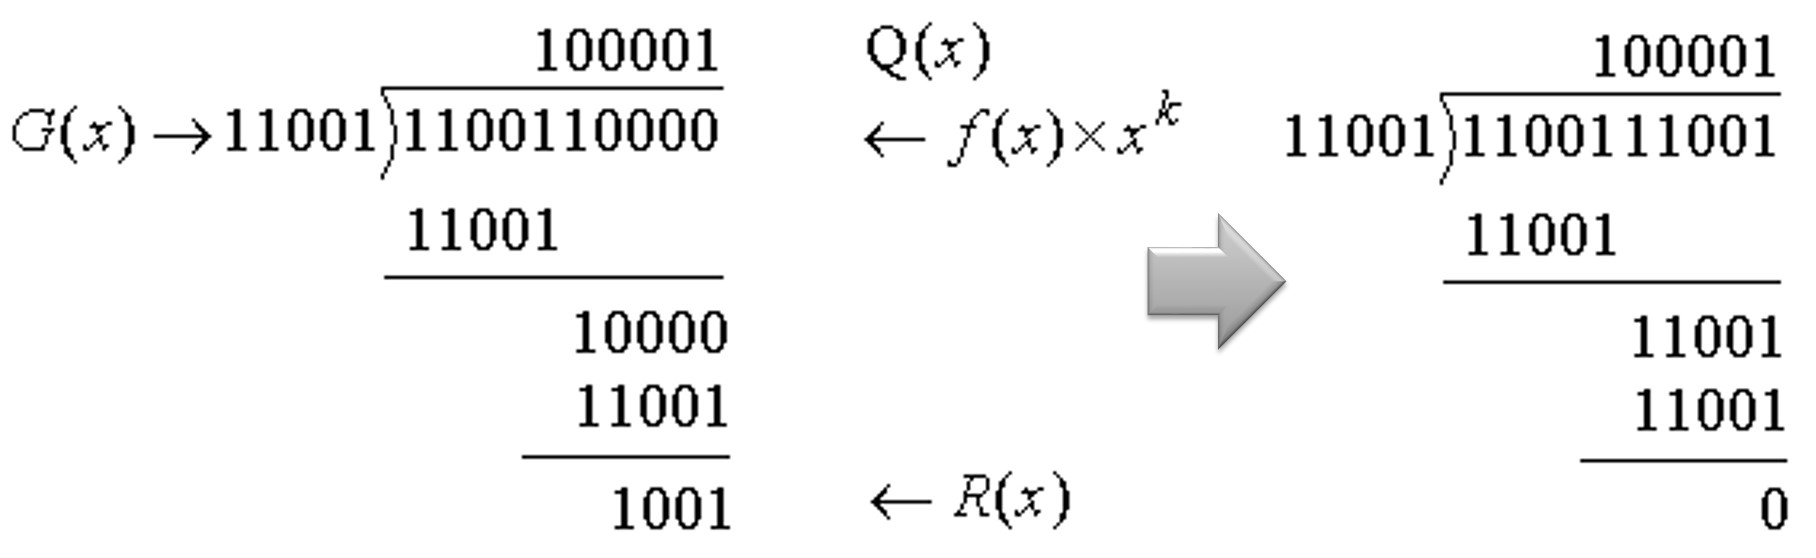
\includegraphics[width=0.6\textwidth]{fig_5_13}\\
  \caption{循环冗余码计算}\label{fig_5_13}
\end{figure}
\end{center}



\end{description}


\begin{remark}
  校验码的意义在于检查出错误,但并非可以$100\%$检查出错误。注意如下关系:

  校验错误 $\Rightarrow$ 数据传输错误。

  校验无误 $\Rightarrow$ 数据传输无误?

\end{remark}

\section{本章要点总结}

\begin{itemize}
  \item 数据通信的有效性和可靠性指标;

  \item 了解不同的传输介质,理解介质带宽以及其对信号传输的影响;

  \item 通信线路的工作方式;

  \item 了解信号的基带与载波传输模式,理解调制方法;

  \item 了解各种差错校验方法。

\end{itemize}
